\section{Overview of the Microcode Engine}
- hardware fast\\
- software flexible\\
- microcode engine: basic instructions to gain some amount of flexibility\\

\subsection{Instruction Set}
- table: isa\\
- short description of instructions\\

\subsection{Hardware Architecture}

- 4 pipeline stages\\
- in-order\\
- interfaces\\
- image: black box / stages\\

\subsubsection{Instruction Memory}

- stores the instructions\\
- write interface\\
- 4kx32bit ram\\

\subsubsection{Program Counter}

- address pointer of the current instruction\\
- value is read each clock cycle\\
- updated to point to the next instruction\\
- control flow instruction can modify the pc\\
- execution starts at 'start' signal\\
- execution ends at STOP instruction

\subsubsection{Call Stack}

- stack that can hold up to 14 addresses\\
- CALL pushes address\\
- RET pops address\\
- overflow is passed to external interface\\
- overflow terminates program execution\\
- only stores pc, not scratchpad\\

\subsubsection{Scratchpad}

\begin{figure}[htb]
 \centering
 %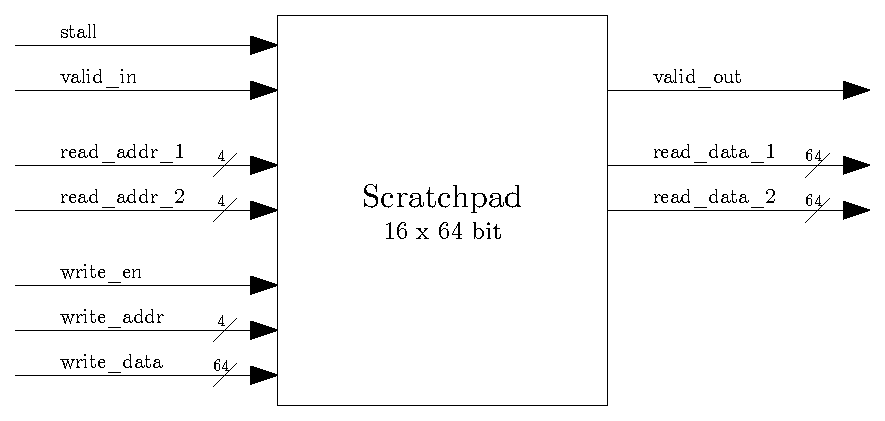
\includegraphics[width=1.0\textwidth,angle=0]{images/scratchpad_blackbox}
 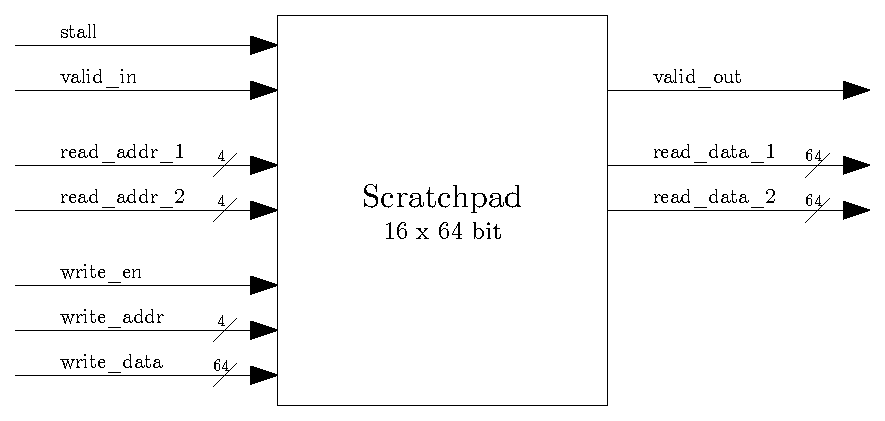
\includegraphics[scale=1.0]{images/scratchpad_blackbox}
 \caption{Scratchpad Interface}
\label{fig:scp_inf}
\end{figure}

- stores results of operations\\
- provides operands to operations\\
- data available next clk cycle\\
- 16x64bit register\\
- 4 bit address\\
- 1 write port (stage 3)\\
- written by ALU and memory interface\\
- 2 read ports (stage 1)\\
- data forwarding when same address is read/written\\


\subsubsection{Arithmetic Logic Unit}

- executes operations\\
- calculates results\\
- calculates condition code\\
- stage 2\\

\subsubsection{Memory Interface}

- access to the registerfile\\
- LDR read from memory\\
- STR write to memory\\
- stalls pipeline, when read/write conflict occurs\\
- stalls pipeline, when memory access, while pending access\\
- stage 2\\

\subsubsection{Condition Code Register}

\begin{figure}[htb]
 \centering
 %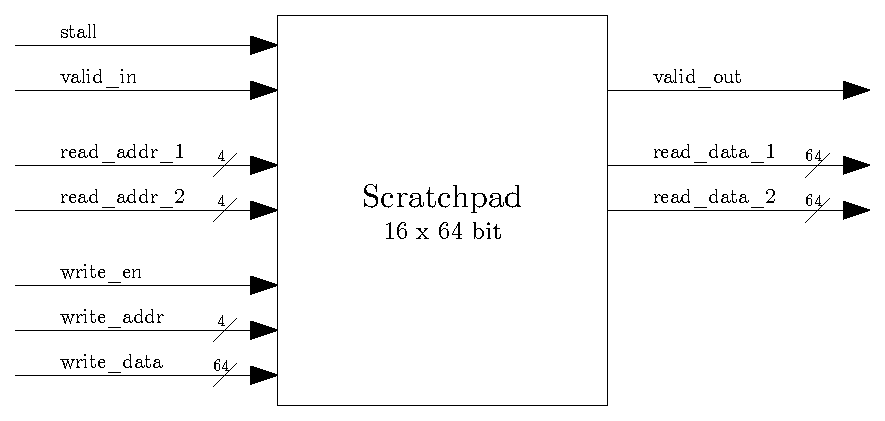
\includegraphics[width=1.0\textwidth,angle=0]{images/scratchpad_blackbox}
 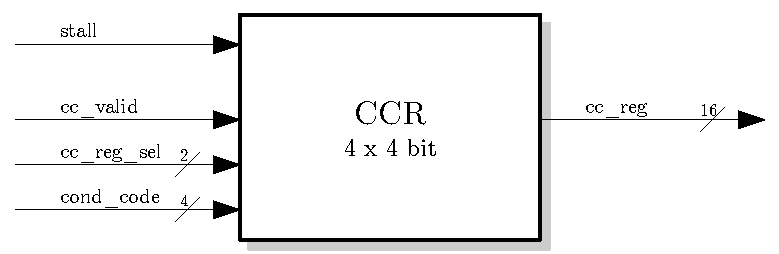
\includegraphics[scale=1.0]{images/ccr_blackbox}
 \caption{Condition Code Register Interface}
\label{fig:scp_inf}
\end{figure}

- 4x4bit register\\
- stores condition code calculated by ALU\\
- only written by ALU\\
- each bit can be accessed directly to determine, if a GUARD instruction or BCC should be executed\\
- stage 3\\
- 3 instructions delay between writing and reading instruction\\




